\documentclass[14pt,russian,a4paper]{extarticle}

\usepackage[a4paper,left=30mm,right=15mm,top=20mm,bottom=20mm,bindingoffset=0cm]{geometry}
\usepackage{amsfonts,amssymb,amsmath,enumerate,float}
\usepackage{cmap}
\usepackage{ifthen}
\usepackage[utf8]{inputenc}
\usepackage[T2A]{fontenc}
\usepackage[russian]{babel}

\usepackage{graphicx}
\usepackage[font=small,labelfont=bf]{caption}
\usepackage{hyperref}
\usepackage{titlesec}


\newcommand{\gb}[1]{\guillemotleft #1\guillemotright}

\renewcommand{\labelitemi}{$\bullet$}
\renewcommand{\labelitemii}{$\circ$}
\renewcommand{\labelitemiii}{$\diamond$}

\titleclass{\subsubsubsection}{straight}[\subsection]

\newcounter{subsubsubsection}[subsubsection]
\renewcommand\thesubsubsubsection{\thesubsubsection.\arabic{subsubsubsection}}
\renewcommand\theparagraph{\thesubsubsubsection.\arabic{paragraph}} % optional; useful if paragraphs are to be numbered

\titleformat{\subsubsubsection}
  {\normalfont\normalsize\bfseries}{\thesubsubsubsection}{1em}{}
\titlespacing*{\subsubsubsection}
{0pt}{3.25ex plus 1ex minus .2ex}{1.5ex plus .2ex}

\makeatletter
\renewcommand\paragraph{\@startsection{paragraph}{5}{\z@}%
  {3.25ex \@plus1ex \@minus.2ex}%
  {-1em}%
  {\normalfont\normalsize\bfseries}}
\renewcommand\subparagraph{\@startsection{subparagraph}{6}{\parindent}%
  {3.25ex \@plus1ex \@minus .2ex}%
  {-1em}%
  {\normalfont\normalsize\bfseries}}
\def\toclevel@subsubsubsection{4}
\def\toclevel@paragraph{5}
\def\toclevel@paragraph{6}
\def\l@subsubsubsection{\@dottedtocline{4}{7em}{4em}}
\def\l@paragraph{\@dottedtocline{5}{10em}{5em}}
\def\l@subparagraph{\@dottedtocline{6}{14em}{6em}}
\makeatother

\setcounter{secnumdepth}{4}
\setcounter{tocdepth}{4}


\linespread{1.5}

\begin{document}

\thispagestyle{empty}

{\footnotesize 

\begin{center}
    МИНИСТЕРСТВО ОБРАЗОВАНИЯ И НАУКИ РОССИЙСКОЙ ФЕДЕРАЦИИ \\
    ФЕДЕРАЛЬНОЕ ГОСУДАРСТВЕННОЕ АВТОНОМНОЕ ОБРАЗОВАТЕЛЬНОЕ \\
    УЧРЕЖДЕНИЕ ВЫСШЕГО ОБРАЗОВАНИЯ \\
    \guillemotleft НОВОСИБИРСКИЙ НАЦИОНАЛЬНЫЙ ИССЛЕДОВАТЕЛЬСКИЙ ГОСУДАРСТВЕННЫЙ \\
    УНИВЕРСИТЕТ\guillemotright (НОВОСИБИРСКИЙ ГОСУДАРСТВЕННЫЙ УНИВЕРСИТЕТ, НГУ)
\end{center}

\vspace{4mm}

\begin{flushleft}
    Факультет {\bf ФИЗИЧЕСКИЙ} \\
    Кафедра {\bf ФИЗИКО-ТЕХНИЧЕСКОЙ ИНФОРМАТИКИ}
\end{flushleft}
\begin{flushleft}
    Направление подготовки {\bf 03.04.02 ФИЗИКА} \\
    Образовательная программа {\bf МАГИСТРАТУРА}
\end{flushleft}

\vspace{4mm}


\begin{center}
    {\bf
    ВЫПУСКНАЯ КВАЛИФИКАЦИОННАЯ РАБОТА \\
    МАГИСТЕРСКАЯ ДИССЕРТАЦИЯ
    }
\end{center}

\begin{center}
    {\bf Герасёв Алексей Владимирович}
\end{center}

\begin{center}
    Тема работы: {\bf Разработка системы управления быстрыми компонентами электронно-лучевой установки}
\end{center}

\vspace{4mm}

\leftline{\bf \gb{К защите допущена}}

\vspace{2mm}

\noindent
\begin{minipage}[t]{70mm}
    \begin{center}
    {\bf Заведующий кафедрой} \\
    учёная степень, звание \\
    должность, место работы \\
    Логашенко И. Б. / \makebox[20mm]{\dotfill} \\
    \gb{\makebox[10mm]{\dotfill}} \makebox[30mm]{\dotfill} 20\makebox[5mm]{\dotfill} г.
    \end{center}
\end{minipage}
\hfill
\begin{minipage}[t]{70mm}
    \begin{center}
    {\bf Научный руководитель} \\
    к.т.н., \\
    с.н.с., ИЯФ СО РАН \\
    Болховитянов Д. Ю. / \makebox[20mm]{\dotfill} \\
    \gb{\makebox[10mm]{\dotfill}} \makebox[30mm]{\dotfill} 20\makebox[5mm]{\dotfill} г. \\
    м.н.с., ИЯФ СО РАН \\
    Чеблаков П. Б. / \makebox[20mm]{\dotfill} \\
    \gb{\makebox[10mm]{\dotfill}} \makebox[30mm]{\dotfill} 20\makebox[5mm]{\dotfill} г.
    \end{center}
\end{minipage}

\vspace{4mm}

\begin{flushright}
    Дата защиты: \gb{\makebox[10mm]{\dotfill}} \makebox[30mm]{\dotfill} 20\makebox[5mm]{\dotfill} г.
\end{flushright}

\vfill

\centerline{Новосибирск, 2018}
}

\newpage
\thispagestyle{empty}
\tableofcontents
\newpage

\section{Введение}

\subsection{Электронно-лучевые технологии}
В последнее время электронно-лучевые технологии всё шире используются в науке и промышленности. Принцип работы основан на том, что мощный пучок электронов попадает на материал объекта, помещённого в вакуум, и локально нагревает его до высоких температур. Данный подход используется для точной резки и сварки металлов, в том числе химически активных, тугоплавких и разнородных. Так как есть возможность получить достаточно узкий пучок высокой мощности, данная технология позволяет добиться высокой точности обработки материала. Также с недавнего времени широкое развитие получают такие направления электронно-лучевых технологий как аддитивные (к которым относится трёхмерная печать) и ионно-плазменные.

\subsection{Электронно-лучевые установки в ИЯФ}
В настоящее время в Институте Ядерной Физики СО РАН ведутся работы по развитию электронно-лучевых технологий \cite{weld_coord}. В ИЯФ СО РАН были разработаны, собраны и запущены несколько электронно-лучевых установок. Одна из этих установок (так называемая "малая" установка) является экспериментальной и используется для разработки и изучения новых электронно-лучевых технологий. При разработке малой установки был применён ряд уникальных технических решений (например, альфа-магнит \cite{alpha_magnet} и лазерный подогрев катода \cite{laser_heat}), а также проведён ряд уникальных экспериментов (3D-печать вольфрамом \cite{wolfram_3d} и т.д.).

\section{Малая электронно-лучевая установка}
Данная работа проводится для малой электронно-лучевой установки, поэтому рассмотрим эту установку подробнее.

\subsection{Описание}
Малая электронно-лучевая установка состоит из электронно-оптической колонны с альфа-магнитом \cite{alpha_magnet}, присоединённой к вакуумной камере, куда помещаются объекты, подвергаемые воздействию электронного пучка. Электронный пучок может иметь энергию электронов в диапазоне от 60 кэВ до 150 кэВ при мощности пучка от единиц до нескольких десятков киловатт. \cite{facility_desc} Минимальная ширина пучка при этом составляет около 0.1 мм.
\begin{figure}[h!]
    \centerline{\includegraphics[width=300pt]{media/alpha_scheme.jpeg}}
    \caption{Основные блоки малой электронно-лучевой установки}
    \label{fig:facility}
\end{figure}
\newline
Компоненты установки изображены на рисунке рис. \ref{fig:facility}. Электронная пушка испускает пучок электронов, который проходит через систему магнитной оптики, включающей в себя магнитное зеркало, также называемое альфа-магнитом, магнитные линзы и стигматоры, после чего попадает в технологический объём, где находится объект, подвергаемый воздействию электронного пучка. На данной установке реализована система дифференциальной откачки, что означает, что электронно-оптическая часть установки и технологический объём, сообщаются узким отверстием, которого достаточно только для прохождения узкого электронного пучка, а также каждый имеет собственную систему вакуумных насосов. Сделано это по причине того, что в технологическом объёме происходит активное испарение нагреваемого материала, который потом осаждается на стенки вакуумной камеры, поэтому чтобы как можно сильнее снизить загрязнение чувствительного оборудования и выполнены вышеописанные модификации. Электронная пушка также имеет ещё и собственный турбомолекулярный насос, так как для генерации пучка нужен более высокий вакуум. Альфа-магнит, поворачивающий электронный пучок на 270 градусов, также помогает снизить степень загрязнения источника электронов, так как позволяет переместить его в сторону от выхода из технологического объёма. Также, тот факт, что электронная пушка теперь направлена не в сторону технологического объёма, в будущем может позволить реализовать лазерный подогрев источника электронов, разместив источник лазерного излучения напротив электронной пушки.

\subsection{Модуль управления и контроля}
Модуль управления и контроля находится рядом с установкой, выполнен в виде шкафа в конструктиве "Вишня". В шкафу два верхних этажа занимает модуль УБС (устройство блокировок и сигнализаций), который обеспечивает таймирование управления модуляцией величины тока пучка, измерение токооседания и контроль вакуума. Следующие два этажа занимает модуль питания и контроля катушек магнитной фокусировки и отклонения пучка. Он включает в себя блоки компьютерного управления и контроля восьми каналов питания катушек – прецизионный аналого-цифровой контроллер CAC208 \cite{kozak_cac208}, общение с которыми осуществляется по шине CAN \cite{can}. В этом же шкафу размещается блок оптических связей OSF1, превращающий электрические сигналы в оптические (и обратно) для связи с контроллером прикатодной электроники (такое преобразование необходимо по причине того, что электроника в голове колонны находится под потенциалом -60 кВ). К OSF1 подключена шина CAN, также на него подаются сигналы включения/выключения и модуляции пучка, которые генерируются устройствами, также управляемыми по шине CAN.
\subsubsection{Медленные подсистемы}
Большинство подсистем данной установки, такие как контроль источников питания, блок управления, блокировок и сигнализаций (УБС), часть прикатодной электроники и блока фокусировки и отклонения пучка и другие, не требуют быстрого управления, то есть частота подачи сигналов и время реакции на события может принимать значение порядка нескольких секунд, с чем успешно справляется персональный компьютер. Такие подсистемы мы называем медленными.
\subsubsection{Быстрые подсистемы}
Однако для проведения некоторых экспериментов на установке появилась необходимость в достаточно быстром и точном управлении интенсивностью электронного пучка, магнитной оптикой или перемещении объектов в вакуумной камере. Эти системы мы теперь называем быстрыми.
\newline
Контроль пучка состоит из управления параметрами источника пучка (такими как ток пучка, напряжение на обкладках и т.д.) и магнитной оптикой (фокусировка и отклонение пучка). Контроль данных подсистем осуществляется с помощью аналого-цифрового контроллера CAC208, общение с которым осуществляется по шине CAN. Данное устройство работает с частотой дискретизации 100 Гц.
\newline
Работа "Применение Xenomai для управления технологическим процессом электронно-лучевой сварки" \cite{xeno_weld} была посвящена управлению магнитной оптикой на данной установке в режиме реального времени. Однако после монтажа альфа-магнита на установку, возможный угол отклонения пучка с помощью магнитных линз значительно уменьшился с нескольких десятков сантиметров до единиц, поэтому возникла потребность в механических подвижках, на которых закреплялся бы объект и перемещался бы внутри рабочего объёма. Возникла задача конструирования данных подвижек и разработки системы управления для них.

\newpage

\section{Постановка задачи}
\subsection{Цель работы}
В рамках данной работы была поставлена задача разработать и собрать программно-аппаратную систему управления для быстрых компонентов малой электронно-лучевой установки ИЯФ СО РАН, удовлетворяющую поставленным требованиям, которые описаны далее.

\subsection{Требования к системе управления}
К системе управления был предъявлен список требований, часть которых обусловлена свойствами техпроцесса, часть - экспериментальным характером установки.
\subsubsection{Основные требования}
Система управления должна обеспечивать позиционирование и перемещение механических подвижек по трём осям с обратной связью в виде концевиков (датчиков приближения подвижки к краям оси) внутри электронно-лучевой установки. Желательно, чтобы перемещение осуществлялось по достаточно сложным траекториям, задаваемым пользователем. Также системе управления необходимо уметь работать с CAN-оборудованием на установке. Система управления должна иметь пользовательский интерфейс.
\subsubsection{Быстродействие}
Техпроцесс электронно-лучевых технологий предъявляет следующие требования:
\begin{itemize}
    \item максимальная скорость перемещения подвижек - не менее 10 мм/c;
    \item точность позиционирования - порядка минимальной ширины электронного пучка, равной 0.1 мм;
    \item cинхронизация между каналами - должна удовлетворять предыдущему требованию, то есть не должна вносить ошибку больше ширины пучка - 0.1 мм;
    \item периодичность CAN-посылок - не реже, чем каждые 10 мс.
\end{itemize}
\subsubsection{Гибкость и простота разработки}
Так как малая электронно-лучевая установка в ИЯФ является экспериментальной, то есть на ней проверяются новые технические решения и методы техпроцесса, то желательно чтобы система управления была как можно более многофункциональной и универсальной, и при этом простой в разработке и внесении дальнейших модификаций.

\newpage

\section{Решение задачи}
\subsection{Возможные решения}
Были рассмотрены следующие варианты:
\begin{itemize}
    \item обыкновенный персональный компьютер:
    \begin{itemize}
        \item под управлением стандартной ОС;
        \item под управлением специализированной операционной системы реального времени;
    \end{itemize}
    \item одноплатный микрокомпьютер:
    \begin{itemize}
        \item NI MyRIO\cite{myrio};
        \item Raspberry Pi\cite{raspberry_pi}:
        \begin{itemize}
            \item под управлением стандартной ОС;
            \item под управлением ОС реального времени;
        \end{itemize}
    \end{itemize}
    \item микроконтроллер;
    \item ПЛИС.
\end{itemize}
Рассмотрим каждый из этих вариантов.
\newline
Современные персональные компьютеры с процессором архитектуры x86-64 обладают хорошей производительностью, однако обычно не оборудованы низкоуровневыми аппаратным интерфейсами, которые требуются для работы с оборудованием установки. Это может быть исправлено установкой аппаратных модулей, но они вносят дополнительную сложность. Персональные компьютеры предназначены для работы под управлением операционных систем общего назначения, таких как Linux, Windows и т.д. Эти операционные системы в среднем обладают небольшим временем отклика, однако в редких случаях могут возникать значительные задержки.
\newline
Чтобы избежать этих задержек используются операционные системы жёсткого реального времени. Такие системы гораздо менее функциональные, и, что значительно хуже, с ними совсем не совместимо программное обеспечение, написанное для ОС Linux, используемое в ИЯФ. Однако существует фреймворк для разработки и запуска приложений, называемый Xenomai\cite{xenomai}, который внедряет в ядро Linux небольшую систему реального времени, и позволяет запускать программы для Linux, с небольшими изменениями, в режиме реального времени. Работа "Применение Xenomai для управления технологическим процессом электронно-лучевой сварки" \cite{xeno_weld} была посвящена исследованию и применению Xenomai для этой же электронно-лучевой установки. Однако с Xenomai возникают некоторые трудности. Одна из них - отсутствие драйверов реального времени для большинства устройств. Так как ядро реального времени Xenomai сильно отличается от ядра Linux, требуется разрабатывать отдельные драйвера для необходимых устройств, что является очень трудоёмкой задачей. Другая проблема заключается в том, что архитектура современных ПК не предназначена для жёсткого реального времени, поэтому, например, в случае использования дискретного графического процессора, могут возникать непредвиденные задержки и при использовании ядра Xenomai.
\newline
Другой вариант - использовать компьютеры с другой архитектурой, например, одноплатные компьютеры. Был рассмотрен вариант компьютера National Instruments MyRIO\cite{myrio}. Он имеет необходимые нам аппаратные интерфейсы, а также, что очень хорошо, работает на базе чипа Xilinx Zinq, который имеет помимо процессора ARM ещё и FPGA (ПЛИС) на борту. Однако основными проблемами данной платформы является её закрытость, использование собственного программного интерфейса и средств разработки, что делает очень сложной задачу переноса используемого в ИЯФ программного обеспечения на данную платформу. Также можно отметить высокую стоимость данного решения.
\newline
Другой одноплатный компьютер, рассмотренный нами - Raspberry Pi\cite{raspberry_pi}. В отличие от предыдущей платформы, Raspberry Pi является открытой, использует свободную операционную систему Debian Linux, очень много готовых программ и библиотек с открытой документацией, стандартный для Linux программный интерфейс, и огромное сообщество разработчиков. Raspberry Pi может использоваться в качестве компьютера общего назначения. Данный компьютер, также, как и MyRIO, имеет много низкоуровневых аппаратных интерфейсов. Также можно отметить высокую доступность данного компьютера и большое количество различных плат расширения для него.
\newline
Также была исследована возможность использования Xenomai для Raspberry Pi, было собрано ядро Linux для Raspberry Pi с Xenomai, однако оказалось, что Xenomai ещё не умеет должным образом работать с периферией Raspberry Pi вследствие чего возникают различные ошибки, плюс остаётся проблема с драйверами для Xenomai.
\newline
Были рассмотрены варианты использования микроконтроллеров и ПЛИС (Программируемые Логические Интегральные Схемы). Данные устройства обеспечивают очень высокое быстродействие в режиме жёсткого реального времени. Однако разработка, отладка и внесение модификаций программы для данных устройств имеет высокую сложность.
\newline
Из всех вышеперечисленных вариантов была выбрана платформа Raspberry Pi, как удовлетворяющая всем требованиям к системе управления и наиболее удобная для разработки и использования программного обеспечения.

\subsection{Raspberry Pi}
\subsubsection{Обзор платформы}
Raspberry Pi - это полноценный одноплатный компьютер. Внешний вид этого компьютера изображён на рис. \ref{fig:rpi_front} и \ref{fig:rpi_back}. Существуют несколько версий и моделей данной платформы, но нас интересуют версии 2 и 3, которые являются наиболее производительными и близки друг к другу по функционалу.
\newline

\begin{figure}[h!]
    \centerline{\includegraphics[width=400pt]{media/rpi_layout_front.jpg}}
    \caption{Одноплатный компьютер Raspberry Pi 3, вид сверху}
    \label{fig:rpi_front}
\end{figure}

\begin{figure}[h!]
    \centerline{\includegraphics[width=400pt]{media/rpi_layout_back.jpg}}
    \caption{Одноплатный компьютер Raspberry Pi 3, вид снизу}
    \label{fig:rpi_back}
\end{figure}

Компьютер работает на базе процессора архитектуры ARM\cite{arm}. Версии 2 и 3 имеют на борту 1 ГБ оперативной памяти LPDDR2.
Операционная система загружается с MicroSD флеш-накопителя, для которого имеется разъём на плате, и в дальнейшем работает с файловой системой на этом накопителе.
\newline
Для питания требуется источник питания напряжением 5 В, обеспечивающий ток до 2.5 А. Питание подключается либо ко входу MicroUSB на плате, либо к GPIO, однако имеется информация, что второй вариант нежелателен, так как не оборудован защитами, как первый\cite{raspberry_pi_power}.
\newline
Raspberry Pi может использоваться как полноценный персональный компьютер, либо как встраиваемое устройство.

\subsubsection{CPU и SoC}
Raspberry Pi - это система на кристалле (System on Chip, SoC) - то есть на основном чипе находится не только центральный процессор (Central Processing Unit, CPU), но и другие подсистемы платформы. 
Версия 2 использует чип Broadcom BCM2836, работающий на базе 64-битного процессора ARM\cite{arm} Cortex-A7 (система команд ARMv7-A), имеющего 4 процессорных ядра и работающего на частоте 900 МГц.
Версия 3 - чип BCM2837 с также 64-битным процессором ARM Cortex-A53 (ARMv8-A) - 4 ядра, 1.2 ГГц. Помимо центрального процессора на кристалле расположен  графический процессор (Graphics Processing Unit, GPU) - VideoCore IV, работающий на частоте 250 МГц в версии 2 и 400 МГц в версии 3 и также имеющий доступ к оперативной памяти. Архитектура системы на кристалле\cite{raspberry_pi_peripherals} у всех версий Raspberry Pi практически совпадает, и помимо центрального и графического процессора включает в себя:
\begin{itemize}
    \item таймеры;
    \item контроллер прерываний;
    \item GPIO (Ввод-вывод общего назначения);
    \item USB;
    \item PCM / I2S;
    \item контроллеры DMA;
    \item I2C master + I2C slave;
    \item 3 SPI + 1 SPI slave;
    \item PWM (ШИМ);
    \item 2 UART.
\end{itemize}
Также имеется ряд модулей, используемых графическим процессором, однако не рекомендуется работать с ними через центральный процессор.
Все периферийные устройства, а также центральный и графический процессор имеют доступ к общей шине, и взаимодействуют друг с другом через неё. Шина представлена как адресное пространство. Иерархия адресных пространств Raspberry Pi изображена на рис. \ref{fig:rpi_mem}.

\begin{figure}[h!]
    \centerline{\includegraphics[width=400pt]{media/rpi_mem.png}}
    \caption{Структура адресных пространств компьютера Raspberry Pi}
    \label{fig:rpi_mem}
\end{figure}

Программы на Raspberry Pi работают с виртуальным адресным пространством, на которое отображено физическое адресное пространство с помощью ARM MMU (Memory Management Unit - менеджер памяти). На физическое адресное пространство отображается адресное пространство шины посредством ARM MMU и VideoCore MMU. На адресное пространство шины отображаются периферийные устройства, а также оперативная память (SDRAM). Адресное пространство шины поделено на четыре одинаковых области, которые отличаются только двумя старшими битами, которые определяют способ кэширования при записи в эту память. Работа с оборудованием осуществляется посредством записи и чтения из области адресов, принадлежащих шине.
Raspberry Pi версии 2 и 3 имеют следующие внешние интерфейсы:
\begin{itemize}
    \item 4 USB 2.0;
    \item 40 GPIO контактов;
    \item Ethernet 10/100 Mbps;
    \item HDMI;
    \item 3.5 мм аудиовыход (совмещённый с композитным видеовыходом);
    \item последовательные интерфейсы камеры (CSI) и дисплея (DSI).
\end{itemize}
Версия 3 имеет дополнительно:
\begin{itemize}
    \item 802.11n Wireless LAN;
    \item Bluetooth 4.0.
\end{itemize}

\subsubsection{Операционная система}
Для Raspberry Pi доступен набор операционных систем начиная от различных версий и дистрибутивов Linux и заканчивая Windows 10 IoT Core. Для нашей системы управления был выбран Raspbian\cite{raspbian} - порт дистрибутива Debian Linux специально для Raspberry Pi с поддержкой математического сопроцессора (архитектура armhf - ARM hardware float). Этот выбор был сделан по причине того, что Linux - современная открытая операционная система, лучше всего подходящая для разработки и исполнения программ, а Raspbian является основной сборкой Linux для Raspberry Pi с наилучшей поддержкой и содержит на данный момент 35 000 из более чем 50 000 доступных пакетов Debian, портированных под Raspberry Pi.

\subsubsection{Разработка приложений}
Существует два способа разработок приложений для Raspberry Pi - прямой и кросс-компиляция. Кросс-компиляция - способ, когда приложение разрабатывается и собирается на другой машине, часто с другой архитектурой, на которую устанавливается набор библиотек и компиляторов для целевой архитектуры, и только уже собранная программа загружается на нужную машину. Второй способ - когда разработка и сборка происходит непосредственно на целевой машине и для неё. В нашем случае для сборки программной части системы управления мы использовали прямой способ, так как он гораздо более простой и удобный, наша система управления имеет достаточно небольшой объём программного кода, а Raspberry Pi является полноценным компьютером, подходящим в том числе и для таких задач. Однако, для сборки более объёмных программных компонент, например, для сборки Linux, нам приходилось использовать кросс-компиляцию, так как процессоры ARM на данный момент всё ещё уступают по производительности процессорам настольных компьютеров архитектуры x86-64.

\subsection{Система управления}
Разработка системы управления состояла из двух частей: аппаратной и программной.
\subsubsection{Аппаратная часть}
Разработка аппаратной части включала в себя выбор и изучение оборудования для управления системами установки, организация и настройка связи между этим оборудованием и компьютером Raspberry Pi, а также размещение всего этого в стандартном конструктиве.

\subsubsubsection{Управление шаговыми двигателями}

\begin{figure}[h!]
    \centerline{\includegraphics[width=300pt]{media/axes.jpg}}
    \caption{Внешний вид подвижек}
    \label{fig:axes}
\end{figure}

Система подвижек состоит из трёх осей, каждая из которых приводится в движение шаговым двигателем посредством винтового механизма. Внешний вид подвижек в собранном состоянии изображён на рис. \ref{fig:axes}. В данных подвижках используются шаговые двигатели FL42STH производства НПФ Электропривод\cite{stepper}. Внешний вид двигателя приведён на рис. \ref{fig:stepper}.
\newline
Шаговые двигатели в рассматриваемой установке управляются по протоколу \gb{step-dir} через трёхканальный драйвер шаговых двигателей SMD-303 производства НПФ Электропривод \cite{stepper_driver} (изображён на рис. \ref{fig:stepper_driver}).
\newline

\begin{figure}[h!]
    \centerline{\includegraphics[width=300pt]{media/fl42sth.jpg}}
    \caption{Внешний вид шагового двигателя FL42STH}
    \label{fig:stepper}
\end{figure}

\begin{figure}[h!]
    \centerline{\includegraphics[width=400pt]{media/smd-303.jpg}}
    \caption{Внешний вид драйвера шаговых двигателей SMD-303}
    \label{fig:stepper_driver}
\end{figure}

На каждый двигатель на драйвере приходится по три цифровых входа: \gb{step}, \gb{dir}  и \gb{enable}. Вход \gb{dir} отвечает за направление вращения двигателя: когда на него подаётся логический ноль - двигатель вращается против часовой стрелки, а когда единица - по часовой стрелке. Когда на вход \gb{step} подаётся импульс - двигатель делает один шаг. Вход \gb{enable} включает или отключает ток через обмотки двигателя. Когда двигатель стоит, этот вход включает или отключает режим удержания. Сигналы на данные входы подаются напрямую с GPIO Raspberry Pi.
\newline
В нашей системе используется довольно простой механизм перемещения шагового двигателя, характеризующийся тремя параметрами: начальной скоростью, максимальной скоростью и максимальным ускорением. Начальная скорость - это такая скорость, с которой двигатель может начать двигаться из состояния покоя сразу, без разгона. Максимальная скорость - наибольшая скорость, до которой двигатель может стабильно разогнаться. Максимальное ускорение - наибольшее ускорение, с которым двигатель может разгоняться. Механизм передвижения таков: двигатель стартует с начальной скорости, разгоняется с постоянным максимальным ускорением до максимальной скорости, движется с этой скоростью почти до нужного положения, после чего с таким же ускорением тормозит до начальной скорости и останавливается. На стадию разгона и торможения приходится фиксированное число шагов, остальные шаги двигатель проходит с постоянной скоростью. Если нужно сделать меньше шагов, чем требуется для разгона и торможения в сумме, то первую половину пути двигатель разгоняется с максимальным ускорением, не достигая максимальной скорости, вторую половину пути тормозит с таким же ускорением.
Примерный график скорости при данном механизме движении приведён на рис. \ref{fig:stepper_move}.

\begin{figure}[h!]
    \centerline{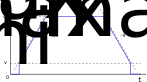
\includegraphics[width=400pt]{media/stepper_move.pdf}}
    \caption{Характерный график зависимости скорости от времени при перемещении подвижки. $v$ - скорость двигателя, $t$ - время, $v_{ini}$ - начальная скорость, $v_{max}$ - максимальная скорость, $a_{max}$ - максимальное ускорение двигателя.}
    \label{fig:stepper_move}
\end{figure}

Все возможные виды движения двигателей в нашей системе реализуются только через протокол \gb{step-dir}, то есть последовательностью импульсов с плавно меняющейся частотой. Точность позиционирования подвижек обусловлена в первую очередь точным подсчётом выдаваемых импульсов, а также правильно подобранными параметрами движения, при которых шаги не пропускаются двигателем.

\subsubsubsection{Расчёт перемещения}
Приведём пример расчётов периода импульсов для перемещения подвижки.
Допустим, нам нужно быстро переместить подвижку на $N$ шагов. Согласно вышеописанному методу перемещения, мы должны сперва плавно ускорить подвижку до максимальной скорости, проехать с этой скоростью, а потом плавно остановиться. Соответственно, перемещение делится на три этапа: ускорение, движение с постоянной скоростью, торможение. Рассчитаем сколько шагов нам нужно сделать на каждом этапе. Пусть параметры двигателя следующие: $v_i$ - начальная, $v_m$ - максимальная скорости в шаг$/c$, $a_m$ - максимальное ускорение шаг$/c^2$.
\newline
$$
\tau_a = \frac{v_m - v_i}{a_m}
$$
$\tau_a$ - время разгона подвижки до максимальной скорости (и торможения тоже).
$$
N_a = (v_i + a_m \tau_a) \tau_a = v_m \tau_a 
$$
Мы получили $N_a$ - число шагов, которое необходимо сделать, чтобы разогнаться (и затормозить). Соответственно, на этапе движение с постоянной скоростью количество шагов будет равно $N_v = N - 2 N_a$. Однако возможна такая ситуация, когда $N < 2 N_a$, то есть двигатель не успеет разогнаться, а ему уже нужно тормозить. В таком случае перемещение делится на два этапа: ускорение за $N_a^* = \frac{N}{2}$ шагов и торможение за столько же шагов. Если число шагов нечётное, то округляем $N_a$ вниз и дубируем последний шаг после ускорения. Максимальная скорость в таком случае будет равной $v_m^* = \sqrt{v_i^2 + 2 a_m N_a^*}$.
\newline
Теперь, когда мы знаем, сколько шагов нужно сделать на кждом из этапов, можно посчитать задержку на каждом шаге. При движении с постоянной скоростью всё просто - задержка равна $t = \frac{1}{v_m}$. При разгоне задержки рассчитываются сложнее:
$$
t_i = \frac{t_0 t_{N_a} \sqrt{2 N_a}}{\sqrt{2 (N_a - i) t_0^2 + 2 i t_{N_a}^2}}
$$
$t_i$ - задержка при разгоне на шаге $i$. Задержки на первом и последнем шаге равны $t_0 = 1/v_i$ и $t_{N_a} = 1/v_m$ соответственно.

\subsubsubsection{Получение сигнала с сенсоров}

\begin{figure}[h!]
    \centerline{\includegraphics[width=200pt]{media/sensor_mounted.jpg}}
    \caption{Внешний вид сенсора Panasonic GX-F12A-P, смонтированного на ось подвижки.}
    \label{fig:sensor_mounted}
\end{figure}

\begin{figure}[h!]
    \centerline{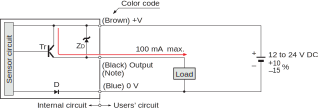
\includegraphics[width=400pt]{media/sensor-circuit.pdf}}
    \caption{Схема сенсора Panasonic GX-F12A-P и механизм подключения.}
    \label{fig:sensor_circuit}
\end{figure}

Каждая ось подвижек оборудована двумя бесконтактными индукционными сенсорами близости модели Panasonic GX-F12A-P. Когда подвижка оказывается на уровне сенсора, металлическая пластинка на подвижке приближается к нему на расстояние в несколько миллиметров, и сенсор срабатывает. Схема сенсора, а также внешний вид и размещение на подвижках изображены на рис. \ref{fig:sensor_circuit}, \ref{fig:sensor_mounted}. 
\newline
Так как сенсоры используются непосредственно в вакуумной камере и подвержены значительным наводкам от электронного пучка, а также работают на напряжении, значительно большем 3.3В, использующихся в логике GPIO, поэтому был разработан и собран адаптер для концевиков с оптической развязкой. Внешний вид и схема приведена на рис. \ref{fig:adapter} и \ref{fig:adapter_circuit}.
\newline

\begin{figure}[h!]
    \centerline{\includegraphics[width=300pt]{media/adapter.jpg}}
    \caption{Внешний вид разработанного нами адаптера концевиков с оптической развязкой.}
    \label{fig:adapter}
\end{figure}

\begin{figure}[h!]
    \centerline{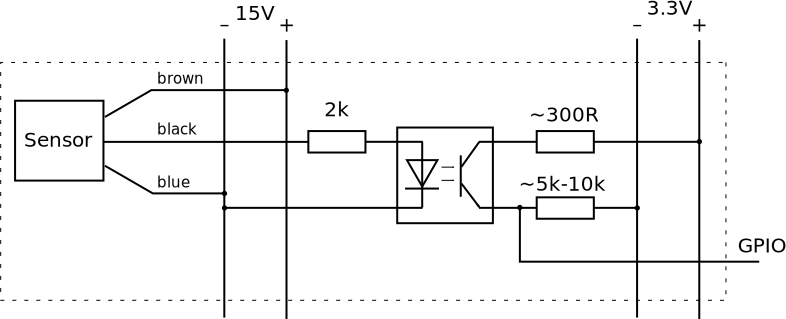
\includegraphics[width=400pt]{media/adapter_scheme.pdf}}
    \caption{Схема элемента адаптера для подключения сенсора к Raspberry Pi с оптической развязкой. На адаптере размещёно 6 таких элементов, следовательно он позволяет подключить 6 сенсоров.}
    \label{fig:adapter_circuit}
\end{figure}

Механизм работы адаптера следующий: когда оптопара закрыта, на входе GPIO - логический ноль. Когда концевик активирован, фотодиод в оптопаре открывается, напряжение на входе GPIO становится +3.3В - то есть логическая единица для GPIO.

\subsubsubsection{Подбор параметров движения}
Был разработан и реализован механизм подбора параметров перемещения подвижки, близких к оптимальным. Проверка параметров работает следующим образом: подвижка перемещается на достаточное расстояние от концевика, после чего движется с новыми параметрами обратно к нему. Если параметры превысили допустимые значения, то подвижка пропустит шаги, остановится и не сможет доехать до концевика. Сперва подбирается начальная скорость. Подбор начинается с некоторой безопасной скорости, с которой двигатель точно сможет ехать. Потом эта скорость последовательно удваивается и проверяется вышеуказанным методом, пока на каком-либо шаге проверка окажется неудачной - то есть начальная скорость превысит допустимое значение. После этого между неудачным и последним удачным значением параметра выполняется несколько шагов двоичного поиска с таким же методом проверки. В результате мы получаем близкое к оптимальному значение скорости и для большей надёжности уменьшаем его на 25\%. После подбора начальной скорости нужно подобрать максимальную скорость и максимальное ускорение. Это сделать сложнее, так как эти параметры зависят друг от друга. Примерный вид зависимости был определён экспериментально и изображён на рис. \ref{fig:stepper_velacc}.
\newline

\begin{figure}[h!]
    \centerline{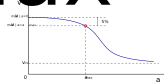
\includegraphics[width=400pt]{media/stepper_velacc.pdf}}
    \caption{Характерный график зависимости максимальной скорости шагового двигателя от ускорения. $v$ и $a$ - скорость и ускорение двигателя в какой либо момент времени, $v_{max | a=0}$ и $v_{max | a=a_{max}}$ - максимальная скорость при условии, что ускорение равно 0 и найденному нами близкому к оптимальному ускорению соответственно.}
    \label{fig:stepper_velacc}
\end{figure}

Был предложен следующий метод поиска данных параметров: берутся некоторые безопасные значения данных параметров. Сначала фиксируется ускорение и выполняется двоичный поиск максимальной скорости также, как и для начальной скорости. Найденное значение запоминается. После этого максимальное ускорение удваивается, снова фиксируется, и снова повторяется поиск максимальной скорости как и на предыдущем шаге, но уже для нового значения ускорения. Попытка подбора некоторого значения ускорения считается удачной, если значение максимальной скорости для этого ускорения не меньше, чем 95\% от максимальной скорости для начального ускорения. Таким образом выполняем также двоичный поиск для значения ускорения, и в результате мы должны получить значение максимального ускорения и соответствующее ему значение скорости не меньше, чем 95\% от максимальной скорости двигателя при начальном ускорении. Данный метод удобен потому, что он почти не требует контроля со стороны человека - только указание начальных безопасных значений параметров. Также он позволяет автоматизированно пересчитывать параметры в случае изменения нагрузки на подвижки или при изменении их конфигурации.

\subsubsubsection{Общение с CAN-устройствами}
У Raspberry Pi нет встроенного CAN-интерфейса, поэтому для общения с оборудованием по шине CAN пришлось использовать внешний CAN-контроллер PICAN2 Duo Iso, который общается с Raspberry Pi по шине SPI и имеет два оптически изолированных CAN-интерфейса. Внешний вид модуля изображён на рис. \ref{fig:pican}. Модуль удобным способом крепится сверху платы Raspberry Pi и соединяется с ней сквозными контактами. Способ крепления модуля в нашей установке изображён на рис. \ref{fig:pican_mounted}.

\begin{figure}[h!]
\centering
\begin{minipage}[t]{180pt}
    \centering
    \includegraphics[height=160pt]{media/pican2duo.png}
    \captionof{figure}{Внешний вид CAN-контроллера PICAN2 Duo Iso}
    \label{fig:pican}
\end{minipage}%
\hspace{20pt}
\begin{minipage}[t]{180pt}
    \centering
    \includegraphics[height=160pt]{media/pican_mounted.jpg}
    \captionof{figure}{Способ крепления CAN-контроллера PICAN2 Duo Iso поверх компьютера Raspberry Pi}
    \label{fig:pican_mounted}
\end{minipage}
\end{figure}

Данный CAN-контроллер работает на базе микросхемы MCP2515, для которой в операционной системе Raspberry Pi имеется драйвер, позволяющий управлять ей через стандартный интерфейс SocketCAN, что очень удобно, так как это даёт возможность использовать на Raspberry Pi большой набор готовых библиотек для CAN-устройств.

\subsubsubsection{Конструктив}

\begin{figure}[h!]
\centering
\begin{minipage}[t]{200pt}
    \centering
    \includegraphics[width=200pt]{media/box.jpg}
    \captionof{figure}{Расположение аппаратных компонент внутри корпуса}
    \label{fig:box}
\end{minipage}%
\hspace{20pt}
\begin{minipage}[t]{200pt}
    \centering
    \includegraphics[width=200pt]{media/box_back.jpg}
    \captionof{figure}{Задняя панель корпуса}
    \label{fig:box_back}
\end{minipage}
\end{figure}

Всё это оборудование вместе с блоками питания было размещено в корпус, устанавливаемый в 19'' стойку (на рис. \ref{fig:box}). На передней панели имеется только кнопка включения питания.
Задняя панель изображена на рис. \ref{fig:box_back}. На ней расположены (слева направо): три четырёхконтактных разъёма для подключения шаговых двигателей, DB-9 разъём для подключения концевиков, DB-9 разьём для подключения к шине CAN. Далее расположено отверстие, напротив которого размещен компьютер  Raspberry Pi так, чтобы наружу смотрели порт Ethernet и 4 USB порта. Далее находятся плавкие предохранители, по одному на блоки питания 5 В и 12-24 В, и разъём для подключения сетевого кабеля 220 В с заземлением.

\subsubsection{Программная часть}
Программная часть системы управления представляет из себя многоуровневую систему, где каждый вышестоящий уровень (слой) работает на более высоком уровне абстракции. Примерная схема изображена на рис. \ref{fig:rpicnc_stack}.
\newline

\begin{figure}[h!]
    \centerline{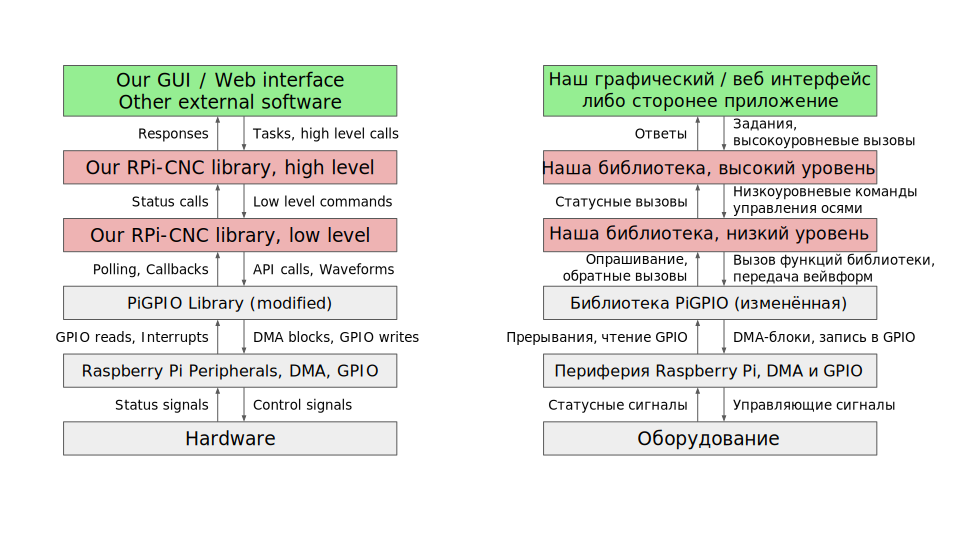
\includegraphics[width=300pt]{media/rpicnc_stack.pdf}}
    \caption{Схема уровней компонент программной части системы управления}
    \label{fig:rpicnc_stack}
\end{figure}

\begin{itemize}
    \item На самом верхнем уровне находится графический Web-интерфейс пользователя. Он позволяет выполнять высокоуровневые задания и отображает текущее состояние системы.
    \item Уровнем ниже находится разработанная нами библиотека RPi-CNC, которая делится высокоуровневую и низкоуровневую части:
    \begin{itemize}
        \item Высокоуровневая часть библиотеки обрабатывает задачи, полученные от пользователя, и преобразует их в низкоуровневые команды. Также она преобразует данные полученные с нижнего уровня в формат, удобный для отображения в графическом интерфейсе.
        \item Низкоуровневая часть синхронизирует низкоуровневые команды от вышестоящего слоя и преобразует их в последовательность цифровых импульсов, которые передаются нижестоящему слою - библиотеке PiGPIO. Также эта часть библиотеки опрашивает состояние оборудования - также через библиотеку PiGPIO.
    \end{itemize}
    \item Как было сказано выше, между библиотекой RPi-CNC и аппаратной частью платформы Raspberry Pi находится сторонняя библиотека PiGPIO, которая предоставляет удобный интерфейс для работы с нижестоящим уровнем.
    \item Дальше идут периферийные подсистемы Raspberry Pi: системная шина, контроллеры DMA, PWM. Они выполняют команды, сформированные библиотекой PiGPIO, и выдают сигналы непосредственно на цифровые выходы GPIO, которые соединены с внешним оборудованием аппаратной части системы управления, таким как контроллер шаговых двигателей или адаптер концевиков.
\end{itemize}
Рассмотрим сейчас подробнее компоненты библиотеки и программные сущности, которыми она оперирует, а также некоторые аппаратные компоненты платформы Raspberry Pi.

\subsubsubsection{GPIO}
GPIO (General Purpose Input and Output - входы и выходы общего назначения) - физический  разъем на плате компьютера Raspberry Pi, а также аппаратные системы управляющие выводом и считыванием сигналов на этих контактах. Внешний вид контактов и схема их расположения и функций изображены на рис. \ref{fig:gpio_pins} и \ref{fig:gpio_pinout} соответственно.
\newline

\begin{figure}[h!]
    \centerline{\includegraphics[width=300pt]{media/gpio_pins.jpg}}
    \caption{Внешний вид контактов GPIO на плате Raspberry Pi}
    \label{fig:gpio_pins}
\end{figure}

\begin{figure}[h!]
    \centerline{\includegraphics[width=400pt]{media/gpio_pinout.png}}
    \caption{Схема расположения и функций контактов GPIO}
    \label{fig:gpio_pinout}
\end{figure}

\subsubsubsection{Вейвформы}
Цифровая вейвформа (waveform) - это последовательность изменений уровня цифрового выхода через определённые промежутки времени. Вейвформа может быть многоканальной, то есть содержать такую последовательность для каждого из нескольких цифровых каналов. На рис. \ref{fig:waveform} изображён пример вейвформы для двух каналов.
\newline

\begin{figure}[h!]
    \centerline{\includegraphics[width=400pt]{media/waveform_example.pdf}}
    \caption{Пример цифровой вейвформы для двух каналов}
    \label{fig:waveform}
\end{figure}

Вейвформы используются в нашей системе управления для формирования последовательностей управляющих импульсов для контроллера шаговых двигателей. Они формируются программно библиотекой RPi-CNC и выдаются на GPIO с помощью подсистемы DMA на Raspberry Pi.

\subsubsubsection{Использование DMA}
DMA (Direct Memory Access - прямой доступ к памяти) - механизм, когда внешние устройства могут работать с оперативной памятью компьютера напрямую, не обращаясь к центральному процессору. DMA в Raspberry Pi - это 16 отдельных устройств на кристалле. DMA-контроллер работает с DMA-блоками. DMA-контроллер, получая такой блок, копирует определённое в блоке количество байт из адреса для чтения в адрес для записи, а после этого переходит к выполнению следующего блока, адрес которого указан в текущем блоке. Все адреса являются адресами в физическом адресном пространстве. Таким образом, блоки можно соединять в цепочки и передавать для выполнения DMA-контроллеру. Устройство DMA-блоков и принцип соединения их в цепочки изображено на рис. \ref{fig:dma_chain}. Так как в Raspberry Pi внешние устройства отображены на физическую память, DMA может также управлять ими. 

\begin{figure}[h!]
    \centerline{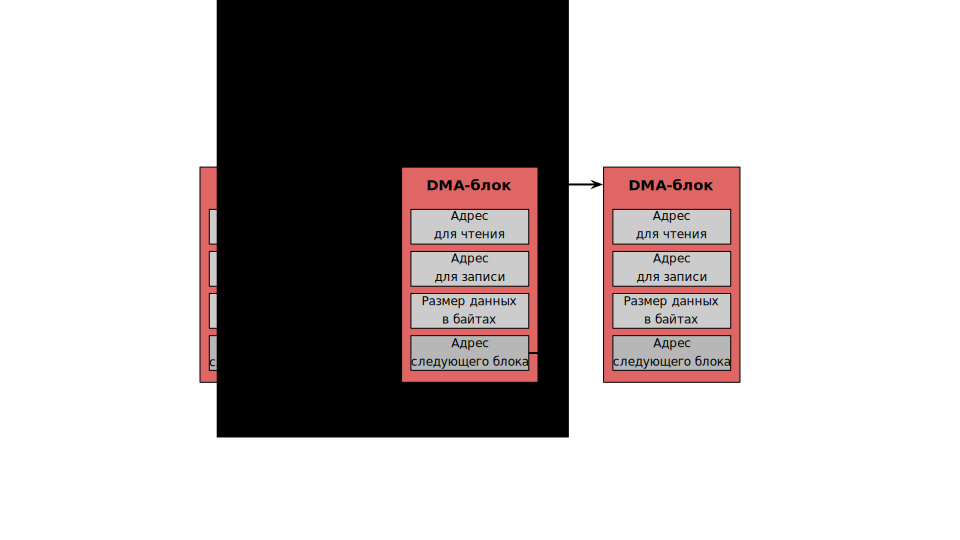
\includegraphics[width=400pt]{media/dma_chain.pdf}}
    \caption{Устройство DMA-блоков и принцип соединения их в цепочку.}
    \label{fig:dma_chain}
\end{figure}

Для создания возможности задержки DMA на заданное время, используется PWM-контроллер (Pulse Width Modulation - Широтно-Импульсная Модуляция, ШИМ), который находится также на чипе. Контроллер может работать в режиме сериализации, когда он выдаёт на один из выходов GPIO сериализованную версию заданного 32-битного слова на заданной частоте. Слова могут браться из специальной очереди внутри этого модуля, которая заполняется с помощью DMA, причём когда очередь заполнена, PWM-модуль посылает сигнал PANIC, который приостанавливает соответствующий DMA-модуль. Когда очередь освобождается, посылается сигнал DREQ (Data REQuest - запрос данных), который возобновляет работу DMA. Таким образом, регулируя частоту и заполняя очередь PWM с помощью DMA, можно реализовать ожидание в течение произвольного времени между двумя DMA-операциями.
С использованием всего вышеперечисленного становится возможным реализовать воспроизведение произвольных вейвформ с помощью DMA, что и делает библиотека PiGPIO.

\subsubsubsection{Библиотека PiGPIO}
Библиотека PiGPIO [ref] размещена пользователем Joan2937 на GitHub под открытой лицензией \gb{Unlicence}. Библиотека очень обширна и предоставляет удобный интерфейс для работы с большим числом периферийных устройств платформы Raspberry Pi. Как заявлено в документации, библиотека позволяет выполнять:
\begin{itemize}
    \item Аппаратное считывание значений из GPIO 0-31 с периодом от 5 мкс.
    \item Аппаратный ШИМ на всех 0-31 GPIO
    \item Аппаратные серво-импульсы на всех 0-31 GPIO
    \item Прерывания по изменению уровня на 0-31 GPIO с точностью до нескольких микросекунд
    \item Прерывания по таймеру
    \item Чтение/запись значений значений всех GPIO за одну операцию
    \item Чтение, запись, переключение режимов и подтягивание уровня на GPIO
    \item Воспроизведение вейвформ на GPIO с точностью до нескольких микросекунд
\end{itemize}
Аналогов этой библиотеки найдено не было, поэтому было решено использовать именно её для в качестве интерфейса для работы с периферией Raspberry Pi.

\subsubsection{Библиотека RPi-CNC}
Библиотека RPi-CNC (Raspberry Pi Computer Numerical Control) разработана и реализована мной на языках C и Python3. Она свободно доступна на GitHub под лицензией MIT. Исходный код разделён на два модуля:
\begin{itemize}
    \item Модуль на языке C - \url{https://github.com/binp-cnc/librpicnc} - низкоуровневые компоненты библиотеки, плюс часть высокоуровневых и программный интерфейс для языка C;
    \item Модуль на языке Python3 - \url{https://github.com/binp-cnc/rpicnc-host} - часть высокоуровневых компонент и программный интерфейс на языке Python3, плюс веб-сервер и веб-интерфейс. Включает в себя вышеупомянутую часть на языке C как подмодуль.
\end{itemize}

\subsubsubsection{Архитектура}

\begin{figure}[h!]
    \centerline{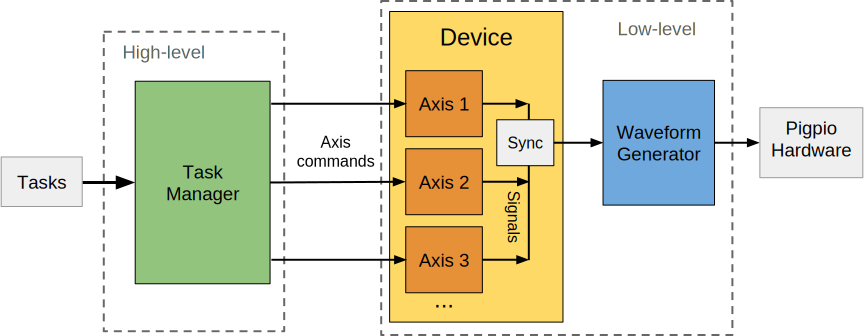
\includegraphics[width=400pt]{media/rpicnc_arch.pdf}}
    \caption{Архитектура библиотеки RPi-CNC}
    \label{fig:rpicnc_arch}
\end{figure}

Упрощённая схема библиотеки изображена на рис. \ref{fig:rpicnc_arch}.
Как было сказано выше, библиотека состоит из низкоуровневой и высокоуровневой части. Рассмотрим эти части.

\subsubsubsection{Низкоуровневая часть}

\begin{figure}[h!]
    \centerline{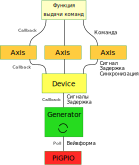
\includegraphics[width=300pt]{media/rpicnc_arch_low.pdf}}
    \caption{Архитектура низкоуровневой части библиотеки RPi-CNC}
    \label{fig:rpicnc_arch_low}
\end{figure}

Низкоуровневая часть нашей библиотеки получает на вход команды для осей, синхронизирует и преобразует их в вейвформы, и отдаёт готовые вейвформы библиотеке PiGPIO для воспроизведения и вывода на GPIO. Данная часть библиотеки работает на принципе обратных вызовов (callbacks), то есть не получает сразу все данные, а запрашивает их по мере необходимости. Составные части представлены на рис. \ref{fig:rpicnc_arch_low}. Названия соответствуют названиям структур в исходном коде библиотеки. Рассмотрим их по порядку:
\begin{itemize}
    \item Generator (генератор) - модуль, отвечающий за сборку вейвформ из последовательностей сигналов и задержек и передачу их библиотеке PiGPIO. Генератор формирует и следит за очередью вейвформ, при необходимости запрашивает данные для новых вейвформ. Запуск генератора является синхронной операцией, поток исполнения заходит в него и находится там, пока вся последовательность данных не выполнится либо не произойдёт принудительная остановка. Сигналы для генератора имеют очень простой вид - это две битовых маски, первая отвечает, какие выходы перевести в состояние логической единицы, вторая - в состояние логического нуля. Сигналы могут разделяться задержками - целое число, означающее паузу между сигналами в микросекундах. Также генератор получает данные с концевиков и осуществляет обратную связь.
    \item Device (устройство) - модуль, олицетворяющий систему подвижек в целом. Отвечает за комбинирование и синхронизацию данных полученных от каждой из осей и передачу их генератору. Формат получаемых данных почти такой же как для генератора, только сигналы и задержки относятся к конкретно каждой из осей, а не ко всей системе подвижек в целом, плюс имеются специальные сигналы, такие как сигнал синхронизации и сигнал окончания списка команд для оси.
    \item Axis (ось) - олицетворяет собой отдельную ось. По мере необходимости получает команды от функции выдачи команд и преобразует их в сигналы, задержки и информацию для синхронизации. Формат возможных команд мы рассмотрим далее. Формат данных, выдаваемых осью, совместим с форматом данных от устройства, поэтому имеется возможность передавать команды от одной оси генератору напрямую, когда необходимо выполнить задание для одной оси (например, такой метод используется для заданий измерения длины оси и подбора оптимальных параметров управления осью).
    \item Функция выдачи команд - функция, определённая пользователем и переданная для обратных вызовов (callbacks). Принимает номер оси и выдаёт следующую команду для этой оси.
\end{itemize}

В общих чертах механизм работы выглядит таким образом - вызывается генератор и получает на вход функцию для обратного вызова, которая возвращает следующий сигнал либо задержку от устройства. Когда вызывается эта функция, устройство запрашивает у каждой из оси следующий сигнал и возвращает тот, который должен произойти следующим по времени. Когда происходит запрос сигнала от оси, она вызывает переданную ей функцию выдачи команд, получает от неё следующую команду и формирует последовательность сигналов и задержек. При следующих запросах ось просто выдаёт по порядку эти сигналы и задержки, пока они не закончатся, и тогда запрашивает у функции выдачи команд новую команду.
Теперь рассмотрим возможные команды для осей:
\begin{itemize}
    \item \detokenize{NONE()} - команда, которая ничего не делает. Когда ось получает такую команду, она просто игнорирует её и запрашивает следующую команду.
    \item \detokenize{IDLE()} - команда, означающая конец списка команд для оси. Когда ось получает такую команду, она переходит в особое состояние, которое говорит устройству, что ей больше нечего выдавать, и устройство её больше не опрашивает.
    \item \detokenize{WAIT(duration)} - команда, означающая задержку на фиксированное количество микросекунд, указанное в поле \gb{\detokenize{duration}}. После выполнения этой задержки устройство будет запрашивать у оси следующие команды.
    \item \detokenize{SYNC(id, count)} - команда, синхронизирующая несколько осей вместе. Содержит поля: \gb{\detokenize{id}} - идентификатор акта синхронизации, и \gb{\detokenize{count}} - количество осей, участвующих в этом акте. Когда ось получает такую команду, она переходит в особое состояние, которое говорит устройству, что для этой оси необходима синхронизация. Когда устройство получает синхросигнал от одной из осей, оно не опрашивает эту ось, пока не получит синхросигнал, имеющий такой же идентификатор \gb{\detokenize{id}}, от других осей, количество которых равно \gb{\detokenize{count}}. После этого устройство вновь начинает запрашивать сигналы от всех этих осей.
    \item \detokenize{MOVE_VEL(dir, steps, period)} - команда перемещения, означающая движение с постоянной скоростью. Направление движения определяется значением поля \gb{\detokenize{dir}}: 1 - движение вперёд, 0 - движение назад. Количество шагов, которые нужно сделать хранится в поле \gb{\detokenize{steps}}. \gb{\detokenize{period}} определяет задержку между шагами микросекундах, то есть величину, обратную требуемой скорости двигателя в шагах в микросекунду.
    \item \detokenize{MOVE_ACC(dir, steps, begin_period, end_period)} - команда перемещения, означающая движение с постоянным ускорением. Поля \gb{\detokenize{dir}} и \gb{\detokenize{steps}} имеют такое же значение, как и в предыдущей команде. Поля \gb{\detokenize{begin_period}} и \gb{\detokenize{end_period}} означают начальный и конечный периоды шагов, соответственно. То есть, данная команда говорит оси разогнаться от начальной скорости, определяемой значением \gb{\detokenize{begin_period}}, до конечной скорости, определяемой значением \gb{\detokenize{end_period}}, с постоянным ускорением за количество шагов равное \gb{\detokenize{steps}}.
    \item \detokenize{MOVE_SIN(dir, steps, begin, size, period)} - команда перемещения по синусоиде в интервале от $-\frac{\pi}{2}$ до $+\frac{\pi}{2}$, на данный момент ещё не реализована, но может быть полезна для движения по эллиптическим траекториям. Поля \gb{\detokenize{dir}} и \gb{\detokenize{step}} имеют те же значения, что и раньше, \gb{\detokenize{size}} означает число шагов во всей синусоиде, \gb{\detokenize{begin}} - с какого шага начинать, \gb{\detokenize{period}} - период шагов в точке 0.
\end{itemize}
Данная часть библиотеки критична по времени, поэтому реализована на языке программирования C и, более того, для большего быстродействия, не использует динамическое выделение памяти в процессе своей работы, только во время инициализации.

\subsubsubsection{Высокоуровневая часть}

\begin{figure}[h!]
    \centerline{\includegraphics[width=300pt]{media/rpicnc_arch_high.pdf}}
    \caption{Архитектура высокоуровневой части библиотеки RPi-CNC}
    \label{fig:rpicnc_arch_high}
\end{figure}

Высокоуровневая часть библиотеки RPi-CNC занимается получением задач, преобразованием их в последовательности команд для осей, и передачей этих команд для выполнения низкоуровневой части. На рис. \ref{fig:rpicnc_arch_high} изображена архитектура высокоуровневой части библиотки вместе с пользовательским интерфейсом. Высокоуровневую часть можно разделить ещё на две компоненты - одна написана на языке C, другая на языке Python3. Часть на языке C, обеспечивающая доступ к низкоуровневым функциям библиотеки, также содержит отдельный поток выполнения, который работает с очередью задач и позволяет асинхронно выполнять их. Задачи принимаются данной частью только в формате последовательности вышеописанных команд плюс некоторые фиксированные задачи. Часть на языке Python частично дублирует интерфейс на C и дополнительно реализует преобразование различных типов задач в необходимый для исполнения формат. Типы задач:
\begin{itemize}
    \item Измерение длины оси (scan) - задача, которая запускает процесс подсчёта шагов от одного концевика до другого, и записывает подсчитанные шаги в свойства оси, которые можно извлечь соответствующим библиотечным вызовом.
    \item Нахождение хороших параметров (calib) - задача запускает процесс нахождения близких к оптимальным параметров движения для оси, описанный выше.
    \item Перемещение из одной точки в другую (move) - наиболее простая задача для перемещения подвижек из одной координаты в другую по прямой. Преобразователь команд вычисляет необходимые значения скорости и ускорения исходя из максимальных значений так, чтобы подвижки перемещались с максимальной возможной скоростью и ускорением, но при этом синхронно двигались по прямой траектории. После этого формируется список команд для осей и передаётся в очередь задач.
    \item Исполнение родных команд (cmds) - задача, не требующая преобразований, содержит список вышеописанных команд для осей, сразу передаётся на выполнение.
    \item Исполнение Gcode (gcode) - задача выполнения Gcode, который является одним из стандартных форматов для управления станками с ЧПУ. Преобразователь команд должен преобразовывать команды Gcode в родные. Данная возможность ещё не реализована.
    \item Движение по кривой (curve) - задача, когда траектория подвижек описывается кривыми Безье. Может быть удобна так как многие компьютерные форматы векторный графики оперируют этими кривыми. Также должна преобразовываться в родные команды. Также ещё не реализована.
\end{itemize}

\subsubsubsection{Пользовательские интерфейсы}
Библиотека RPi-CNC имеет несколько интерфейсов. Два из них - это программные интерфейсы библиотеки для языков C и Python3. Третий - это веб-интерфейс. Программные интерфейсы имеют следующий вид:
\begin{itemize}
    \item \detokenize{init(axes_count, axes_info)} - инициализация библиотеки;
    \item \detokenize{quit()} - деинициализация библиотеки;
    \item \detokenize{clear()} - очистка состояния библиотеки;
    \item \detokenize{run_task(task)} - выполнение задачи в синхронном режиме;
    \item \detokenize{read_sensors()} - считывание показаний сенсоров;
    \item \detokenize{axes_info(axes_info)} - получение информации об осях (длина, положение, номера GPIO-выходов);
    \item \detokenize{push_task(task)} - добавление задачу в очередь задач;
    \item \detokenize{run_async()} - асинхронное выполнение задачи из очереди;
    \item \detokenize{is_busy()} - проверка, выполняется ли какая-либо задача сейчас;
    \item \detokenize{wait()} - ожидание, пока не выполнятся все задачи из очереди;
    \item \detokenize{stop()} - принудительная остановка всех задач.
\end{itemize}
Python-интерфейс имеет дополнительную возможность преобразования задания к стандартному формату системы, а в остальном он и C-интерфейс имеют одинаковые вышеуказанные методы и отличия связаны в основном только со спецификой языка.
\newline

Перейдём к пользовательскому веб-интерфейсу. Веб-интерфейс предназначен для удобного доступа к параметрам системы. На данный момент он имеет доступ далеко не ко всем возможностям, которые предоставляют программные интерфейсы, но с помощью него удобно выполнять простые операции. Данного функционала достаточно для ряда экспериментов, и в дальнейшем функционал интерфейса будет расширяться.

\begin{figure}[h!]
    \centerline{\includegraphics[width=400pt]{media/rpicnc_web.png}}
    \caption{Снимок страницы веб-интерфейса RPi-CNC в браузере}
    \label{fig:rpicnc_web}
\end{figure}

На рис. \ref{fig:rpicnc_web} изображён внешний вид веб-интерфейса системы управления. В верхней части расположена информация о текущем состоянии системы и соединения, информация о выполнении задач и кнопка экстренной остановки. Ниже расположены блоки управления и настроек каждой из осей. В них отображаются текущее положение оси, её измеренная длина, состояния концевиков. Имеются поля ввода для параметров и кнопки запуска измерения длины оси и автоматического подбора параметров. В самом низу находится блок перемещения подвижек. В нём есть графическое поле, где отображается текущее положение и можно указать точку для перемещения. Также присутствуют поля для ввода точного положения подвижек, и кнопка для запуска перемещения.
\newline
Из всех вариантов графических интерфейсов был выбран именно веб-интерфейс по нескольким причинам: большая гибкость такого подхода, лёгкость использования и отсутствие необходимости устанавливать специальные библиотеки (требуется только браузер с поддержкой HTML5 и WebSocket, т.е. почти любой современный браузер), кроссплатформенность.
\newline
Клиентская часть веб-интерфейса работает в браузере на пользовательском компьютере и написана на традиционной для такого подхода связке HTML, CSS и JavaScript. Соединение с серверной частью устанавливается через Ethernet по протоколу HTTP и WebSocket. WebSocket является расширением HTTP и по сути представляет из себя чуть более сложный TCP-сокет. Использование вебсокетов оправдывается тем, что они не закрывают TCP соединение после передачи данных как HTTP-соединение, а остаются открытыми, и клиент и сервер в любой момент могут отправить друг другу сообщение, поэтому вебсокет значительно повышает интерактивность интерфейса.
\newline
Серверная часть работает на Raspberry Pi внутри блока системы управления. С ней устанавливает соединение клиентская часть. Серверная часть представляет из себя веб-сервер, реализованный с помощью асинхронной Python3-библиотеки Aiohttp с поддержкой вебсокетов. Сервер взаимодействует с Python-интерфейсом библиотеки RPi-CNC, передаёт команды от клиента и уведомляет его в случае изменения состояния системы.

\subsubsection{Монтаж на установку}
Для монтажа подвижек в стенке вакуумной камеры были размещены вакуумные разъёмы для двигателей и концевиков, был изготовлен переходник с 18 контактов на 8 (так как каждый из 6 концевиков имеет три контакта - земля, питание и сигнал, при этом первые два из них могут быть объединены). Провода от двигателей и концевиков, которые должны находиться в вакууме, были покрыты металлической оплёткой, чтобы предотвратить накопление заряда на них.
\newline
Корпус с разработанной системой управления подвижками был размещён в шкафу управления и контроля и подключен по Ethernet в локальную сеть оборудования электронно-лучевой установки Взаимодействие с оператором осуществляется посредством персонального компьютера, который также подключен к этой локальной сети.

\subsubsection{Оценка параметров системы}
Было экспериментально получено, что Raspberry Pi позволяет стабильно генерировать импульсы с частотой 10 кГц, при большей частоте иногда происходят задержки. Двигатель FL42STH делает 200 шагов на оборот. Один оборот шагового двигателя перемещает подвижку на 1 мм. Поэтому, чтобы двигать подвижку с требуемой скоростью 10 мм/c, требуется, чтобы двигатель делал 2000 шагов в секунду. Для этого нужно выдавать управляющие импульсы с частотой 2 кГц. Было экспериментально получено, что Raspberry Pi позволяет стабильно генерировать импульсы с частотой 10 кГц, при большей частоте иногда происходят задержки. Следовательно, Raspberry Pi позволяет перемещать подвижки не только с требуемой скоростью, но и со скоростью до 50 мм/c (однако, на деле скорость ограничена шаговым двигателем, и составляет в нашем случае примерно 20 - 30 мм/c).
\newline
Также было было исследовано, насколько синхронно подаются сигналы на разные выходы GPIO. Было получено, что в среднем рассинхронизация составляет 200 нс, в редких случаях до 1 мкс, что примерно на 2 порядка меньше минимального периода сигналов и, соответственно, не вносит почти никакой ошибки. Полученные осциллограммы приведены в приложении.
\newline
Была проведена оценка пространственной точности. Так как система управления может позиционировать подвижки с точностью до шага, то точность позиционирования определяется тоже с точностью до шага, то есть 1/200 мм = 5 мкм. У самих подвижек ошибка позиционирования указана как 20 мкм. Обе эти ошибки меньше минимальной ширины пучка, равной 0.1 мм, поэтому удовлетворяют требованиям к точности позиционирования.

\newpage

\section{Заключение}

\subsection{Полученные результаты}
Были исследованы различные варианты оборудования для системы управления и сделан выбор в пользу платформы Raspberry Pi. Разработана и собрана программно-аппаратная система управления быстрыми компонентами электронно-лучевой установки. Измерены параметры системы, произведён монтаж на установку.

\subsection{Выводы}
Платформа Raspberry Pi является довольно удобным и универсальным инструментом для создания различного рода программно-аппаратных систем, однако имеет свои недостатки. Один из них - это трудность в обеспечении жёсткого реального времени. Платформа отлично подходит для создания прототипов систем управления, однако для промышленного применения лучше использовать более специализированное оборудование.

\subsection{Планы на будущее}
В будущем планируется дорабатывать и развивать данную систему управления в тесном контакте со специалистами, работающими на установке, для достижения наибольшего удобства и функциональности. Планируется также модернизировать аппаратные и программные составляющие. Одно из направлений - введение программно-аппаратного уровня между Raspberry Pi и оборудованием в виде микроконтроллера или ПЛИС. С одной стороны, это значительно улучшит быстродействие и синхронизацию системы управления, что может потребоваться для дальнейших экспериментов на установке, с другой стороны, сохранит лёгкость разработки, так как основным элементом останется Raspberry Pi, а на микроконтроллер или ПЛИС будет перенесена наиболее простая, но критичная ко времени, логика. Другое направление - развитие программной составляющей, включающее в себя настройку коммуникации с другими системами, используемыми в ИЯФ (например, CX\cite{cx}), исследование новых информационных технологий на предмет применимости в такого рода задачах (например, системный язык программирования Rust).

\newpage

\section{Список литературы}

\begin{thebibliography}{99}

\bibitem{weld_coord}
Купер Э.А., Логачев П.В., Репков В.В., Селиванов А.Н., Селиванов П.А., Семенов Ю.И., Трибендис А.Г., Федотов М.Г., Чертовских А.С. -
Автоматизированная система для задания координат шва в установках электронно-лучевой сварки. –
Автометрия. Издательство СО РАН. Новосибирск. – 2015. – Том 51, №1. – С. 55 – 61.

\bibitem{wolfram_3d}
Семенов Юрий Игнатьевич, Алякринский О.Н., Болховитянов Д.Ю., Логачев П.В., Медведев А.М., Спесивцев А.Б., Старостенко А.А., Яминов К.Р. -
Макет 3D принтера для изготовления металлических структур из тугоплавких металлов с помощью электронно-лучевых аддитивных технологий. -
Институт ядерной физики им. Г.И. Будкера СО РАН (Новосибирск), Россия. -
\url{http://conf.ict.nsc.ru/clapt2015/ru/program}

\bibitem{alpha_magnet}
О.Н. Алякринский, М.А. Батазова, Д.Ю. Болховитянов, М.Ю. Косачев, П.В. Логачев, А.М. Медведев, Ю.И. Семенов, М.М. Сизов, А.А. Старостенко, А.С. Цыганов. Прототип источника электронов с магнитным поворотом пучка для электронно-лучевых технологий.

\bibitem{laser_heat}
О.Н. Алякринский, К.В. Губин, М.Ю. Косачев, Э.А. Купер, П.В. Логачев, А.М. Медведев, В.К. Овчар, В.В. Репков, Ю.И. Семенов, М.М. Сизов, А.А. Старостенко, М.Г. Федотов, А.С. Цыганов. Прототип источника пучка электронов с лазерным подогревом катода.

\bibitem{facility_desc}
Энергоблок для установки электронно-лучевой сварки с внутрикамерной электронно-оптической колонной – Краткое описание и инструкция по эксплуатации – \url{https://drive.google.com/open?id=1JrrE1etLfC301fcXQOi6f3ODAfCXQ4m_zBib-fV6Bjk}

\bibitem{xeno_weld}
Герасёв А. В. -
Применение Xenomai для управления технологическим процессом электронно-лучевой сварки : выпускная квалификационная работа бакалавра -
Научный руководитель: Чеблаков П. Б. -
Новосибирск, 2016.

\bibitem{can}
Texas Instruments –
Introduction to Controller Area Network (CAN) –
\url{http://www.ti.com/lit/an/sloa101a/sloa101a.pdf}

\bibitem{kozak_cac208}
Козак Виктор Романович -
Прецизионный аналого-цифровой контроллер CAC208 -
22 мая 2014 г. -
\url{http://www.inp.nsk.su/~kozak/designs/cac208.htm}

\bibitem{myrio}
National Instruments -
MyRIO - учебное устройство для проектирования встраиваемых систем -
\url{http://www.ni.com/ru-ru/shop/engineering-education/portable-student-devices/myrio-student-embedded-device/what-is-myrio.html}

\bibitem{raspberry_pi}
Raspberry Pi - Official Website -
\url{https://www.raspberrypi.org/}

\bibitem{raspbian}
Raspbian -
Операционная система для Raspberry Pi, основанная на базе Debian Linux -
\url{https://www.raspbian.org/}

\bibitem{raspberry_pi_power}
Raspberry Pi Stack Exchange -
How do I supply power through the GPIO? -
\url{https://raspberrypi.stackexchange.com/questions/1617/how-do-i-supply-power-through-the-gpio/1618#1618}

\bibitem{raspberry_pi_peripherals}
Broadcom -
BCM2835 ARM Peripherals -
документация по периферии чипов, использующихся в компьютере Raspberry Pi -
\url{https://www.raspberrypi.org/documentation/hardware/raspberrypi/bcm2835/BCM2835-ARM-Peripherals.pdf}

\bibitem{arm}
ARM Processors -
Official Website -
\url{https://www.arm.com/products/processors}

\bibitem{xenomai}
Xenomai – Real-time framework for Linux –
Official Website -
\url{https://xenomai.org/}

\bibitem{stepper}
НПФ "Электропривод" -
Гибридные шаговые двигатели серии FL42STH -
документация -
\url{http://electroprivod.ru/fl42sth.htm}

\bibitem{stepper_driver}
НПФ "Электропривод" -
Блок управления шаговыми двигателями SMD-303 -
документация -
\url{http://electroprivod.ru/smd-303.htm}

\bibitem{cx}
Болховитянов Д. Ю. –
Программное обеспечение системы управления инжекционного комплекса ВЭПП-5 :
автореферат дис. ... кандидата технических наук :
01.04.01 [Место защиты: Ин-т ядерной физики им. Г.И. Будкера, 2007] -
\url{http://www.inp.nsk.su/news/defences/bolkhovityanov-autoref.pdf}

\end{thebibliography}

\newpage

\section{Приложения}

\end{document}
